\chapter[Referencial Teórico]{Referencial Teórico}
\label{chap:referencialTeorico}

Neste capítulo, será apresentado os conceitos teóricos utilizados como base para o desenvolvimento do catálogo de segurança para o padrão arquitetural MVC.

Antes de entender os conceitos relevantes para o desenvolvimento do catálogo é importante entender a definição de software, e segundo \cite{sommerville2003engenharia}, pode ser entendido como, programas de computador e toda documentação associada. E para realização do desenvolvimento do software da maneira mais correta possível, existe a Engenharia de Software que preocupa-se com todos os aspectos da produção \cite{sommerville2003engenharia}. 

A Figura \ref{BigPicture}, apresenta a visão geral da construção do catálogo, partindo da Engenharia de Software e apoiando principalmente em duas disciplinas: a (i) Engenharia de Requisitos, que compõe-se de um conjunto de tarefas e técnicas que auxiliam a promoção do entendimento dos requisitos, essa disciplina será brevemente detalhada na seção \ref{sec:requisitos}, então, entramos no contexto da orientação à meta, que trata dos requisitos funcionais e não funcionais como metas a serem alcançadas, será detalhado na Subseção \ref{subsec:orientacaoMeta}. Como essa monografia trata dos RNFs, para elaboração do catálogo, logo na Subseção \ref{subsec:requisitosNaoFuncionais} será apresentado conceitos sobre o que são os RNFs. Portando a seção seguinte \ref{sec:NFR} será detalhado o NFR \textit{framework}, para modelar e analisar as interdependências entre os RNFs, e (ii) Desenho de software, uma área da Engenharia de Software que possui como uma de suas preocupações o planejamento e a definição do padrão arquitetural a ser utilizado, os conceitos de arquitetura de software e do padrão arquitetural MVC serão detalhados na seção \ref{sec:arquitetura} e subseção \ref{subsec:mvc}.

\begin{figure}[h!]
	\centering
	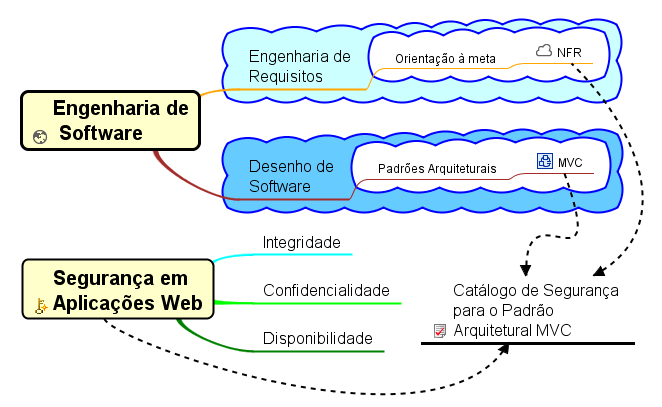
\includegraphics[keepaspectratio=true,scale=0.65]{figuras/bigPicture.png}
	\caption{Visão geral da proposta do catálogo.}
	\label{BigPicture}
\end{figure}

Segundo \cite{chung2012non}, segurança pode ser entendido como a satisfação de três conceitos, e que podem ser interpretados como subtipos : (i) Integridade, (ii) Confidencialidade, (iii) Disponibilidade, e Portanto, o catálogo de segurança é elaborado a partir deles, seguindo a expressão \ref{eq:EstruturaLogicaDeSeguranca}. O conceito de segurança como RNFs, será detalhado na seção \ref{sec:seguranca}

\begin{equation}
	\label{eq:EstruturaLogicaDeSeguranca}
	\textrm{Integridade E Confidencialidade E Disponibilidade SATISFAZ Segurança}
\end{equation}

\section{Engenharia de Requisitos}
\label{sec:requisitos}

Ao conjunto de tarefas e técnicas utilizadas para promover o entendimento dos requisitos é denominado Engenharia de Requisitos \cite{pressman2011engenharia}. No desenvolvimento de software, ela pode ser vista como uma fase importante da Engenharia de Software, que se inicia nas atividades de comunicação com os \textit{stakeholders} e continua até a entrega do produto, sendo adaptada de acordo com as necessidades do processo de desenvolvimento, do produto e dos \textit{stakeholders} \cite{pressman2011engenharia}.

A Engenharia de Requisitos, abrange sete fases distintas: concepção, levantamento, elaboração, negociação, especificação, verificação e validação \cite{pressman2011engenharia}. De acordo com \cite{kotonya1998requirements}, durante a execução das atividades nas fases da Engenharia de Requisitos, alguns problemas são relatados como: (i) os requisitos não refletem as reais necessidades do cliente, de acordo com o sistema a ser desenvolvido; (ii) são inconsistentes e/ou incompletos; (iii) é complexa e possui um custo alto, a realização de alguma mudança no requisito, logo após terem sido acordados entre as partes; e (iv) comumente são interpretados de maneira errada pela equipe de desenvolvimento, diante do que foi solicitado pelo cliente. 


Boa parte dos modelos utilizados na Engenharia de Requisitos não possuem tratamento adequado para lidar com os critérios de qualidade. Logo, o tratamento desses critérios tem sido uma preocupação para a comunidade da Engenharia de Requisitos. Atualmente, existem esforços no sentido de aprimorar os modelos e especificações desses requisitos, e são fortemente associados à comunidade de pesquisadores da Engenharia de Requisitos Orientada à Meta (GORE) \cite{chung2012non}. Nesta monografia, é abordado o uso de uma notação específica para tratar RNFs, proposta por essa comunidade, no caso, trata-se do NFR \textit{framework} \cite{chung2012non}. 

O NFR \textit{framework} é um \textit{Framework} conceitual que procura lidar com os requisitos não funcionais, permitindo especificar os mesmos em um alto nível de abstração e, gradualmente, fornecendo insumos para que essa especificação seja trazida para um nível mais baixo de abstração. Nesse último nível, são especificadas as operacionalizações, as quais evidenciam alternativas para viabilizar a implementação desses requisitos no nível de código. Mais adiante, serão apresentados detalhes dessa notação.

\subsection{Engenharia de Requisitos Orientada à Meta}
\label{subsec:orientacaoMeta}

A Engenharia de Requisitos Orientada à Meta (GORE), tem-se popularizado nos últimos anos e constitui-se do tratamento dos requisitos funcionais e não funcionais, como metas a serem alcançadas \cite{van2001goal}, pois, seus modelos possuem como objetivo a modelagem da razão pela qual determinado requisito existe, essa modelagem, promove ao engenheiro de requisitos uma estratégia mais detalhada do problema, podendo então encontrar uma solução mais adequada \cite{van2001goal}\cite{chung2012non}. O GORE é um paradigma que vem sendo cada vez mais reconhecido para a execução das atividades nas fases da Engenharia de Requisitos \cite{van2001goal}.

Nas definições do GORE, existem as metas que são componentes essenciais, pois de acordo com \cite{van2001goal}, uma meta é definida como propriedades do sistema que são expressas pelos \textit{stakeholders}, através de determinadas questões como, o “\textbf{porquê}” uma meta é exigida, “\textbf{como}” ela pode ser atingida, e “\textbf{quem}” será o responsável pela meta no sistema e no ambiente.

\begin{figure}[h]
	\centering
	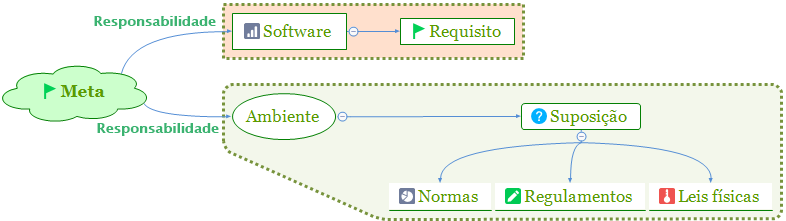
\includegraphics[keepaspectratio=true,scale=0.8]{figuras/GORE.png}
	\caption{Responsabilidades da meta sob o software e sob o ambiente.}
	\label{Gore}
\end{figure}


\pagebreak

 Através da Figura \ref{Gore}, pode-se entender como são os comportamentos das metas no GORE. Representada pelo simbolo de uma nuvem, uma meta, quando está sob a responsabilidade de um único software, essa meta pode-se tornar um requisito, de forma semelhante quando essa meta, está sob responsabilidade de um ambiente, ela pode tornar-se uma suposição, diferente de um requisito as suposições não podem aplicadas pelo software, mas podem ser satisfeitas devido as normas, regulamentos organizacionais e leis físicas \cite{van2001goal}. Esta monografia, possui foco apenas nas responsabilidades voltadas ao software.


Existem diversos \textit{frameworks} orientados à metas, os principais  são o NFR \textit{Framework} \cite{chung2012non} e o i* \cite{istarwiki20}, esses \textit{frameworks} são detalhados nas seções \ref{sec:NFR} e \ref{sec:i*}, respectivamente.

\subsection{Requisitos Não-Funcionais}
\label{subsec:requisitosNaoFuncionais}

A visão do software como um produto, fez com que os aspectos que avaliam a qualidade de um software passassem a possuir maior atenção, e apenas satisfazer, o mais próximo possível de todos os requisitos funcionais não é o suficiente, logo, tem se dado uma atenção maior para os RNFs tais como: Segurança, Integridade, Disponibilidade, etc \cite{cysneiros1997definindo}.

Os RNFs podem ser entendidos como restrições sobre como os requisitos funcionais devem ser implementados, e determinam como o software deve realizar suas funções \cite{sommerville1997requirements}.


Júlio Leite, afirma em sua pesquisa que os RNFs impactam o produto software em qualidade e preço, pois segundo ele:

\begin{citacao}
	"A não observância da necessidade de RNFs durante o processo de desenvolvimento do software, pode levar uma recodificação custosa e demorada o que consequentemente, eleva o preço do software." \cite[p. 2]{cysneiros1997definindo}
\end{citacao}

Os RNFs devem ser analisados em toda sua magnitude para o desenvolvimento e manutenção de um produto de software, sendo importante analisar os possíveis conflitos que podem ser gerados com outros RNFs e com requisitos funcionais, esses conflitos se não identificados em uma fase inicial do processo de desenvolvimento do software podem acarretar em problemas futuros, durante as atividades de implementação e implantação do software \cite{cysneiros1997definindo}. 


As classes de NFRs \cite{eckhardt2016non} podem ser compreendidas como subtipos dos atributos de qualidade da Tabela \ref{AtributosDeQualidade}, onde são definidos de acordo com a \cite{organizacion2011iso}. 

\begin{table}[h!]
	\centering
	\caption{Descrição dos atributos de qualidade. Fonte: \cite{organizacion2011iso}.}
	\label{AtributosDeQualidade}
	\begin{tabular}{|c|c|}
		\hline
		\textbf{\begin{tabular}[c]{@{}c@{}}Atributos de \\ qualidade\end{tabular}} & \textbf{Descrição} \\ \hline
		Funcionalidade & \begin{tabular}[c]{@{}c@{}}É a capacidade do software de promover funções que \\ atendam às necessidades explícitas e implícitas.\end{tabular} \\ \hline
		Segurança & \begin{tabular}[c]{@{}c@{}}É a capacidade do software de apresentar níveis\\ aceitáveis e riscos de danos a pessoas, negócios\\ software, propriedades ou ambiente.\end{tabular} \\ \hline
		Confiabilidade & \begin{tabular}[c]{@{}c@{}}É a capacidade do software de manter o nível de \\ desempenho especificado.\end{tabular} \\ \hline
		Usabilidade & \begin{tabular}[c]{@{}c@{}}É a capacidade do software de ser compreendido,\\ de fácil aprendizagem, operável e atraente ao usuário.\end{tabular} \\ \hline
		Eficiência & \begin{tabular}[c]{@{}c@{}}É a capacidade software de apresentar desempenho\\ apropriado, relativo aos recursos utilizados.\end{tabular} \\ \hline
		Portabilidade & \begin{tabular}[c]{@{}c@{}}É a capacidade software de ser transferido de \\ um ambiente para o outro.\end{tabular} \\ \hline
		Manutenção & \begin{tabular}[c]{@{}c@{}}É a capacidade do software de modificado de forma\\ eficiente e eficaz.\end{tabular} \\ \hline
	\end{tabular}
\end{table}

\pagebreak

\section{NFR Framework}
\label{sec:NFR}

O NFR \textit{Framework}  é um modelo intencional, criado para ajudar engenheiros de software e engenheiros de requisitos a lidarem com requisitos não-funcionais, através de um grafo chamado de \textit{Softgoal Interdependency Graphs} (SIGs). Neste tipo de grafo, os requisitos podem ser analisados, uma vez que o SIG permite uma visão vertical desde a estratégia de alto nível até os detalhes operacionais;  possuindo operadores lógicos AND (E) e OR (OU) que promovem uma melhor tomada de decisão; onde  os RNFs são escritos através de uma notação formal, que permite comprovar a precisão e completude de cada RNF \cite{chung2012non}. 

O \textit{framework} também pode ser orientado por processo, dando suporte às atividades e fases do processo de engenharia de requisitos, e pode ser utilizado como complemento nas abordagens de desenvolvimento de software \cite{chung2012non}.

O NFR \textit{Framework} utiliza o conceito de metas flexíveis, que por definição é uma condição ou um estado no mundo real que deseja ser alcançado, podendo assumir natureza subjetiva, pois, o RNF pode variar de acordo com o julgamento de cada pessoa; e natureza relativa, pois, o RNF pode depender de algum tipo de relação com outro RNF \cite{chung2012non}.

\pagebreak

A notação no SIG para a \textbf{meta flexível} é um símbolo similar ao de uma nuvem, conforme apresentado pela Figura \ref{fig01}. Esse simbolo, possui pequenas variações na forma, que representam uma \textbf{operacionalização} (nuvem em negrito), e também uma \textbf{reivindicação} (nuvem tracejada). Mais adiante na Figura \ref{exemploNFR} é apresentada a decomposição de uma meta flexível em outras metas.  

\begin{figure}[h!]
	\centering
	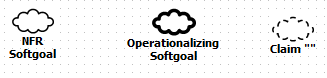
\includegraphics[keepaspectratio=true,scale=0.9]{figuras/tiposDeSoftgoals.png}
	\caption{Representação gráfica dos tipos de metas flexíveis.}
	\label{fig01}
\end{figure} 


Para facilitar no entendimento das decisões tomadas, a meta flexível possui \textit{labels}, que determinam o grau de satisfação para uma meta flexível, de acordo com um conjunto de decisões do projeto. As \textit{labels} são: satisfeita, fracamente satisfeita,  negada, fracamente negada, indecidida e crítica \cite{chung2012non}. Outra notação importante, e que apresenta o grau de prioridade de uma meta flexível, é representado por “\textbf{!}” ou “\textbf{!!}” para um grau de prioridade maior, onde o ponto de afirmação é desenhado a esquerda da nuvem.

\begin{figure}[h]
	\centering
	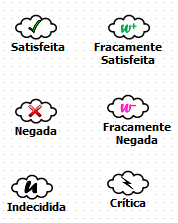
\includegraphics[keepaspectratio=true,scale=0.9]{figuras/labelsSoftgoals.png}
	\caption{Representação gráfica das \textit{labels} em metas flexíveis.}
	\label{fig02}
\end{figure} 

As relações que as metas flexíveis possuem uma com as outras é estabelecida através de \textit{links} de interdependências, sendo esses \textit{links} que realizam o registro da decomposição das metas flexíveis em metas flexíveis mais específicas (filhos). De certa forma, a decomposição em outras metas, contribui para o nível de satisfação da meta flexível mais genérica (pai).

Os \textit{links} de interdependências também podem ser entendidos como tipos de contribuições,e possuem uma notação simbólica para cada tipo, e cada tipo possui um significado, esses tipos de contribuições são apresentados na Tabela \ref{tiposDeContribuições} adaptado de  \cite{chung2012non}.



\begin{table}[h!]
	\centering
	\caption{Tipos de contribuições.}
	\label{tiposDeContribuições}
	\begin{tabular}{|l|l|}
		\hline
		\textbf{Símbolo} & \textbf{Descrição} \\ \hline
		\multirow{2}{*}{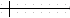
\includegraphics[scale=0.9]{figuras/And.png}} & \multirow{2}{*}{AND: Se todos os filhos são satisfeitos o pai também será satisfeito.} \\
		&  \\ \hline
		\multirow{2}{*}{\includegraphics[scale=0.9]{figuras/OR.png}} & \multirow{2}{*}{OR: Se qualquer filho é satisfeito o pai também será satisfeito.} \\
		&  \\ \hline
		\multirow{2}{*}{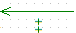
\includegraphics[scale=0.9]{figuras/Make.png}} & \multirow{2}{*}{\begin{tabular}[c]{@{}l@{}}MAKE: Pode ser tratado de forma semelhante ao AND, pois se \\ o filho for satisfeito o pai pode ser satisfeito.\end{tabular}} \\
		&  \\ \hline
		\multirow{2}{*}{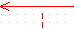
\includegraphics[scale=0.9]{figuras/Break.png}} & \multirow{2}{*}{\begin{tabular}[c]{@{}l@{}}BREAK: Fornece apoio negativo, pois se o filho é satisfeito o \\ pai pode ser negado.\end{tabular}} \\
		&  \\ \hline
		\multirow{2}{*}{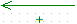
\includegraphics[scale=0.9]{figuras/Help.png}} & \multirow{2}{*}{HELP: Se todos os filhos são satisfeitos o pai também será satisfeito.} \\
		&  \\ \hline
		\multirow{2}{*}{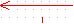
\includegraphics[scale=0.9]{figuras/Hurt.png}} & \multirow{2}{*}{HURT: Se todos os filhos são satisfeitos o pai será fracamente negado.} \\
		&  \\ \hline
		\multirow{2}{*}{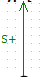
\includegraphics[scale=0.9]{figuras/SomeMais.png}} & \multirow{2}{*}{SOME+: Representa a existência de alguma contribuição positiva.} \\
		&  \\ \hline
		\multirow{2}{*}{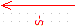
\includegraphics[scale=0.9]{figuras/SomeMenos.png}} & \multirow{2}{*}{SOME-: Representa a existência de alguma contribuição negativa.} \\
		&  \\ \hline
	\end{tabular}
\end{table}

\pagebreak

Os \textit{links} entre as metas flexíveis, representam a contribuição que uma meta flexível tem com outra meta flexível, ou meta flexível de operacionalização, ou meta flexível de reivindicação, logo, a Figura \ref{catalogoDeAvaliação} apresenta a forma como as \textit{labels} são propagadas, de acordo com seu tipo de relacionamento. A propagação das \textit{labels}, se aplica a todos os tipos de metas flexíveis. 

\begin{figure}[h!]
	\centering
	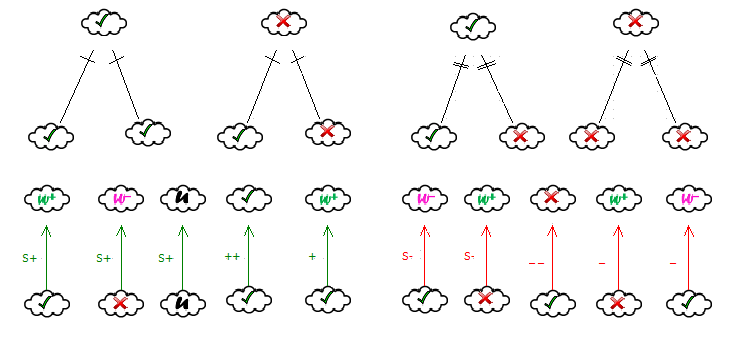
\includegraphics[keepaspectratio=true,scale=0.8]{figuras/catalogoDeAvaliacao.png}
	\caption{Propagação das \textit{labels} para os diferentes tipos de contribuição. Adaptado de \cite{chung2012non}.}
	\label{catalogoDeAvaliação}
\end{figure} 

\pagebreak

A Figura \ref{exemploNFR} apresenta uma decomposição de uma meta flexível em outras metas de mesma natureza. Consideramos, nesse exemplo, o RNF: “manter as contas com boa segurança”. Usando a notação do NFR \textit{Framework}, representou-se a meta flexível  “segurança de contas”, no nível mais generalista do grafo. Em segundo nível, são especificadas as principais metas flexíveis que merecem ser consideradas para que a meta generalista seja "satisfeita", no caso: “Integridade de contas”, “Confidencialidade de contas” e “Disponibilidade de contas” \cite{chung2012non}.

\begin{figure}[h!]
	\centering
	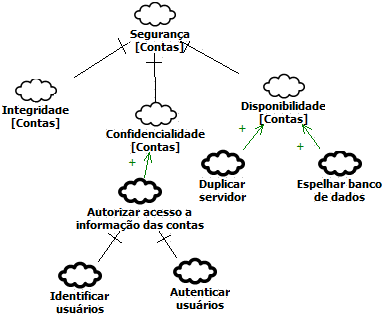
\includegraphics[keepaspectratio=true,scale=1.0]{figuras/exemploNFR.png}
	\caption{Operacionalização de segurança de contas. Adapatado de \cite{chung2012non}, \cite{affleck2012supporting}.}
	\label{exemploNFR}
\end{figure} 

Confidencialidade de contas é operacionalizada em ``Autorizar acesso à informação das contas``, que possui uma contribuição do tipo HELP com seu pai. Dada a relação do tipo AND, entre essa operacionalização e as operacionalizações ``Identificar usuários`` e ``Autenticar usuários``, tem-se que a operacionalização ``Autorizar acesso à informação das contas``  será realizada se ambas as operacionalizações, ``Identificar usuários`` e ``Autenticar usuários``, forem realizadas. Supondo que tudo tenha sido realizado com sucesso, tem-se que esse processo de operacionalização contribui positivamente - HELP (AJUDA) - a atingir ``Confiabilidade de contas``. Como essa meta flexível está especificada em uma relação de AND com as metas flexíveis "Integridade de contas" e ``Disponibilidade de contas``, pode-se dizer que em termos de ``Confiabilidade de contas``, ``Segurança de contas`` tem a ser ``satisfeita``. Mas, resta ainda ponderar se "Integridade de contas" e ``Disponibilidade de contas`` serão de fato ``satisfeitas``. O modelo, da forma como está especificado, não permite avaliar tais aspectos, visto que representa apenas uma visão parcial dessas metas flexíveis.


Para Disponibilidade de contas a mesma é operacionalizada em “Duplicar servidor” e “Espelhar banco de dados” essas operacionalizações possuem contribuições do tipo HELP e mesmo pai, e para a meta flexível ser satisfeita, ambas as operacionalizações devem ser satisfeitas \cite{affleck2012supporting}. 


\section{Framework i*}
\label{sec:i*}


Outra abordagem orientada à meta, o \textit{framework} de modelagem i*\footnote[1]{O nome i* faz referência a utilização da notação de distribuição intencional que é a base do \textit{framework}.}, possui foco em ambientes organizacionais e seus sistemas de informação, tomando como base os relacionamentos de dependência entre os atores participantes \cite{yu1997towards} \cite{istarwiki20}. 

O \textit{framework} é composto por dois modelos; o (i) Modelo de Dependência Estratégica (do inglês, \textit{Strategic Dependency - (SD)}), utilizado para descrever as relações de dependência entre vários atores em um contexto organizacional, e o (ii) Modelo de Razão estratégica (do inglês, \textit{Strategic Rationale - (SR)}), utilizado para descrever os interesses e preocupações das partes interessadas e como eles podem ser abordados pelas configurações do ambiente e dos sistemas \cite{yu1997towards}. Esses dois modelos serão detalhados a seguir nas subseções \ref{subsec:SD} e \ref{subsec:SR}.

Com a utilização do \textit{framework} é possível representar, por meio de seus modelos, os atores participantes e suas dependências, para que suas metas sejam alcançadas, recursos fornecidos, tarefas realizadas e metas flexíveis sejam “satisfeitas a contento” ou “razoavelmente satisfeitas” \cite{istarwiki20}.
 
 
\subsection{Modelo de Dependência Estratégica - SD}
\label{subsec:SD}

O modelo SD é utilizado para expressar através de uma rede de relacionamentos estratégicos e intencionais a relação entre os atores em um contexto organizacional. Em sua modelagem o modelo utiliza um conjunto de nós e ligações, onde cada nó representa um ator e cada ligação entre dois atores indica que um determinado ator depende de outro, para que um objetivo possa ser atingido \cite{istarwiki20}. Os atores e suas dependências podem ser representados de acordo com os símbolos das Figuras  \ref{atoresIstar} e \ref{dependenciaIstar}.

\begin{figure}[h!]
	\centering
	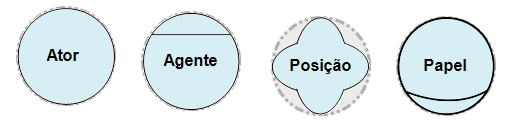
\includegraphics[keepaspectratio=true,scale=1.0]{figuras/papeisIstar.PNG}
	\caption{Símbolos que representam atores no i*.}
	\label{atoresIstar}
\end{figure}

De acordo com as definições de \cite{istarwiki20} um  \textbf{Ator} é o termo utilizado para referir de forma genérica a qualquer unidade em que as dependências intencionais possam ser atribuídas. Os agentes, posições e papeis podem ser entendidos como subunidades de um ator mais complexo e são definidas como: 

\begin{itemize}
	\item \textbf{Agente}: Abstração do comportamento de um ator em algum contexto específico; 
	\item \textbf{Posição}: É definido como um conjunto de funções desempenhadas por um agente, também compreendido como uma abstração intermediária entre um Papel e um Agente, pois pode-se dizer que se um Agente ocupa uma posição essa Posição cobre um papel;
	\item \textbf{Papel}: É definido como manifestações concretas e físicas, utilizado para se referir a humanos e agentes de \textit{Hardware}/\textit{Software}.
\end{itemize} 

No modelo Dependência Estratégica ao existir uma cooperação entre dois atores, essa cooperação é denominada de dependência, onde existe um ``dependente`` (\textit{depender}) e um ``de quem se depende`` (\textit{dependee}), esses atores são ligados por um elo de dependência (\textit{dependum}) que pode ser uma meta a ser atingida, uma tarefa a ser realizada, um recurso a ser fornecido ou uma meta flexível a ser razoavelmente satisfeita \cite{napolitano2009estrategia}. 

\begin{figure}[h!]
	\centering
	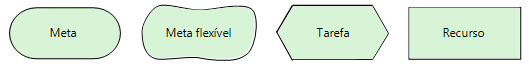
\includegraphics[keepaspectratio=true,scale=1.0]{figuras/TiposDeContribuicao.png}
	\caption{Símbolos que representam o elo de dependência.}
	\label{dependenciaIstar}
\end{figure} 

Os tipos de dependências são definidos por \cite{istarwiki20} como: 

\begin{itemize}
	\item \textbf{Meta}: uma condição ou estado de desejo intencional do ator no mundo real. Os detalhes de como a meta deve ser satisfeita não são descritos, promovendo então a decomposição da mesma em uma série de alternativas.   
	\item \textbf{Meta flexível}: De maneira semelhante a Meta, também representa uma condição ou estado de desejo intencional do ator no mundo real, porém os detalhes de como a meta flexível deve ser satisfeita não são definidos a princípio, sendo então sujeito a interpretação. Para verificar se uma meta flexível foi satisfeita utiliza-se os termos ``satisfeita a contento`` ou ``razoavelmente satisfeita``, pois metas flexíveis não possui critérios claramente definidos. 
	\item \textbf{Tarefa}: Representa a realização de algo em forma particular por um ator. Uma tarefa também pode ser decomposta em subtarefas mais específicas. 
	\item \textbf{Recurso}: Representa uma entidade física ou informativa, presupõe-se então que não existe nenhum problema ou questões abertas sobre como a recurso será alcançado. 
\end{itemize}

A partir das definições dos tipos de dependência e dos atores é possível modelar a relação de dependência entre dois ou mais atores. Como apresentado no exemplo da Figura \ref{exemploTipoDeDepencia}, onde, na modelagem existem dois atores \textbf{Titular do cartão} e \textbf{Banco} e é possível perceber a existência dos 4 tipos de dependência: dependência por recurso, dependência por tarefa, dependência por meta flexível e dependência por meta.  

\begin{figure}[h!]
	\centering
	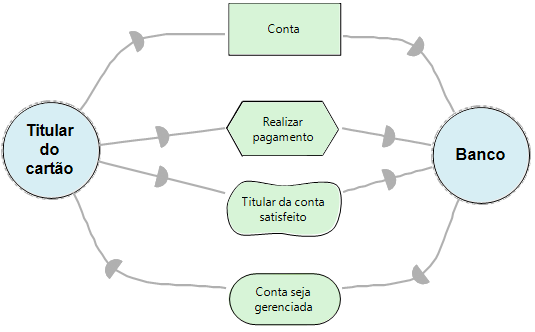
\includegraphics[keepaspectratio=true,scale=1.0]{figuras/ExemploTiposDeDependecias.PNG}
	\caption{Exemplo dos tipos de dependência entre o titular de cartão e o banco.}
	\label{exemploTipoDeDepencia}
\end{figure} 

\begin{itemize}
	\item \textbf{Dependência por recurso}: Neste tipo de dependência, o \textit{depender} depente do \textit{dependee} para que ocorra a disponibilidade do recurso. Ao determinar essa dependência, o \textit{depender} pode utilizar a entidade como um recurso \cite{istarwiki20}. No contexto da figura \ref{exemploTipoDeDepencia}, esse elo existe através do recurso \textbf{conta}, onde o titular do cartão é o \textit{depender} e pode utilizar o recurso da conta bancária.
	
	\item \textbf{Dependência por tarefa}: Neste tipo de dependência, o \textit{depender} depente do \textit{dependee} para realização da tarefa. A tarefa pode ser entendida como uma restrição imposta pelo \textit{depender} ao \textit{dependee}, onde o \textit{dependee} possui certa liberdade de ação dentro dessas restrições \cite{istarwiki20}. No contexto da Figura \ref{exemploTipoDeDepencia}, esse elo existe através da tarefa \textbf{Realizar pagamento}, onde o titular do cartão é o \textit{depender} e ele depende da disponibilização do banco para poder efetuar algum pagamento ao banco. 
	
	\item \textbf{Dependência por meta flexível}: Neste tipo de dependência, o \textit{depender} depente do \textit{dependee} para que alguma tarefa seja realizada para que a meta flexível possa ser "satisfeita a contento" ou "razoavelmente satisfeita" \cite{istarwiki20}. Onde o \textit{depender} determina se a meta flexível será alcançada ou não, utilizando as habilidades e conhecimentos do \textit{dependee} \cite{napolitano2009estrategia}. No contexto da Figura \ref{exemploTipoDeDepencia}, esse elo existe através da meta flexível \textbf{Titular da conta satisfeito}, onde o titular do cartão é o \textit{depender} e ele depende da forma como o serviço do banco é prestado para que o \textit{depender} possa decidir se a meta flexível será alcançada.
	
	\item \textbf{Dependência por meta}: Neste tipo de dependência, o \textit{depender} depente do \textit{dependee} para que um estado no mundo real seja alcançado. O \textit{dependee} possui total liberdade para tomar as decisões necessárias para atingir a meta. O \textit{depender} não se preocupa com o quanto o \textit{dependee} destina-se em satisfazer a meta \cite{istarwiki20}. No contexto da Figura \ref{exemploTipoDeDepencia}, esse elo existe através da meta que a \textbf{Conta seja gerenciada}, onde o banco é o \textit{depender}, pois, espera-se que o titular do cartão tenha capacidade de gerir sua própria conta, através dos recursos fornecidos pelo banco. 
\end{itemize}

\subsection{Modelo de Razão Estratégica - SR}
\label{subsec:SR}

O modelo SR apresenta de forma gráfica, com vários tipos de nós (Meta, Tarefa, Recurso e Meta flexível)\footnote[1]{Os tipos de nós possuem as mesmas definições que os tipos de dependências no Modelo de Dependência Estratégica (SD) descritos na Subseção \ref{subsec:SD}} e links (links de meio-fim, links de decomposição de tarefas e links de contribuição) que servem como estrutura representacional que expressam as razões por trás das dependências \cite{istarwiki20}.

O modelo tem o objetivo principal de representar de forma detalhada as estratégias internas dos atores, em função dos elementos do processo, das alternativas e das decisões por trás do processo, em que as metas são alcançadas, as tarefas são realizadas, os recursos disponibilizados e as metas flexíveis são refinadas e operacionalizadas \cite{napolitano2009estrategia}.  

De acordo com \cite{istarwiki20}, os tipos de \textit{links} são definidos como: 

\pagebreak

\begin{itemize}
	\item \textbf{\textit{link} de meio-fim}: Representado graficamente por uma seta direcionada para o nó fim. O ``\textbf{meio}`` normalmente é expresso por uma tarefa, que define o ``como`` fazer algo e o " \textbf{fim}`` expressa à meta a ser alcançada.
\end{itemize}

\begin{figure}[h!]
	\centering
	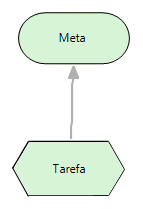
\includegraphics[keepaspectratio=true,scale=0.9]{figuras/meioFim.PNG}
	\caption{Notação gráfica para o \textit{link} de meio-fim, onde, o meio é uma tarefa e o fim é uma meta. Adaptado de \cite{istarwiki20}.}
	\label{meiofim}
\end{figure} 

\begin{itemize}	
	\item \textbf{\textit{link} de decomposição}: Uma tarefa pode ser decomposta em submeta, em subtarefa, em recurso ou em meta flexível. A representação gráfica para um link de decomposição é um segmento de reta com um pequeno corte perpendicular, como apresentado na Figura \ref{decomposicaoLink}.    
\end{itemize}	

\begin{figure}[h!]
		\centering
		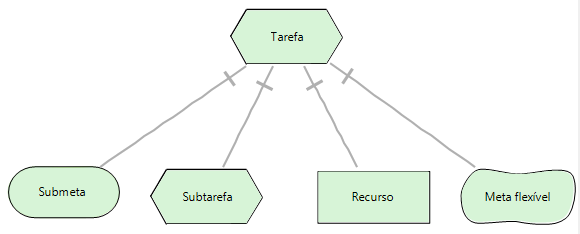
\includegraphics[keepaspectratio=true,scale=1.0]{figuras/decomposicaoLink.PNG}
		\caption{Notação gráfica para o \textit{link} de decomposição. Adaptado de \cite{istarwiki20}.}
		\label{decomposicaoLink}
\end{figure}

\begin{itemize}		
	\item \textbf{\textit{links} de contribuição}: Os tipos de contribuições\footnote[1]{A definição de cada tipo de contribuição é a mesma dada por Chung em \cite{chung2012non}, como visto na Tabela \ref{tiposDeContribuições} que detalha os tipos de contribuições para o NFR Framework.} entre as metas flexíveis são: \textit{Make}, \textit{Some+}, \textit{Help}, \textit{Unknown}, \textit{Break}, \textit{Some-}, \textit{Hurt}, \textit{Or} e \textit{And}. 
\end{itemize}


\section{FURPS}
\label{sec:furps}

O termo FURPS é um acrônimo que define um modelo de atributo de qualidade, esse acrônimo é composto por cinco atributos de qualidade, sendo eles: (i) Funcionalidade (do inglês, \textit{Functionality}), (ii) Usabilidade (do inglês, \textit{Usability}), Confiabilidade (do inglês, \textit{Reliability}), Desempenho (do inglês, \textit{Performance}) e Suportabilidade (do inglês, \textit{Supportability}) \cite{umar2011analyzing}.

\subsection{Funcionalidade}
\label{subsec:funcionalidade}

São os requisitos funcionais de uma aplicação de software, a funcionalidade está diretamente ligada ao comportamento do software e a interação do usuário com o software \cite{cintra2006implementaccao}.

Por definição funcionalidade é a capacidade do software de promover funções que atendam as necessidades explícitas e implícitas quando o software estiver sendo utilizado, de acordo com os cenários especificados \cite{qualidadeDeProdutoNBR}.

\subsection{Usabilidade}
\label{subsec:usabilidade}

A usabilidade faz parte do conjunto dos RNFs de uma aplicação de software, considera-se a experiência do usuário em manipular um computador, a experiência do usuário na utilização do software, estética da interface para o usuário e para o contexto ao qual a aplicação foi desenvolvida \cite{cintra2006implementaccao}.

Por definição usabilidade é a capacidade do software de ser compreendido, aprendido, operado e ser atraente ao usuário, quando o software estiver sendo utilizado de acordo com os cenários especificados \cite{qualidadeDeProdutoNBR}.


\subsection{Confiabilidade}
\label{subsec:confiabilidade}

A confiabilidade faz parte do conjunto dos RNFs de uma aplicação de software, considera-se a prevenção de falhas, capacidade do software se recuperar de um erro, precisão e tempo entre falhas (\textit{Mean Time Between Failure} (MTBF)) \cite{cintra2006implementaccao}.

Por definição confiabilidade é a capacidade do software em manter o nível de desempenho esperado, quando o software estiver sendo utilizado de acordo com os cenários especificados \cite{qualidadeDeProdutoNBR}.  

\subsection{Desempenho}
\label{subsec:desempenho}

O desempenho faz parte do conjunto dos RNFs de uma aplicação de software, considera-se o tempo de recuperação e tempo de resposta do software, a taxa de transferência de dados (do inglês, \textit{troughput}) \footnote[1]{Quantidade de dados que pode ser tranferidos de um lugar para o outro em um espaço de tempo previamente especificado.}, capacidade do software de utilizar os recursos do sistema operacional, etc \cite{cintra2006implementaccao}.

Por definição desempenho é o nível como o software atende as necessidades, representado por um conjunto específico da valores para cada característica especificada para a execução do software. \cite{qualidadeDeProdutoNBR}.  

\subsection{Suportabilidade}
\label{subsec:suportabilidade}

Suportabilidade faz parte do conjunto dos RNFs de uma aplicação de software, considera-se o a capacidade de adaptabilidade, possibilidade de realizar manutenções corretivas e evolutivas, flexibilidade de configuração, flexibilidade de instalação e internacionalização no sistema \cite{cintra2006implementaccao}.

\section{Arquitetura de Software}
\label{sec:arquitetura}

O conceito de design de software surgiu da década de 1970, quando os pesquisadores da época acreditavam que o design fosse uma atividade separada da implementação, exigindo notações, técnicas e ferramentas específicas, foi somente a partir da década de 1990 que utilizou-se o termo arquitetura de software em contraste com design de software, para indicar noções de codificação, abstrações, padrões e treinamentos formais de arquitetos de software \cite{perry1992foundations}.

O termo arquitetura de software é definido por \cite{shaw1996software}, como o entendimento do sistema em termos de seus componentes computacionais e os relacionamentos entre os componentes, os padrões que guiam a composição organizacional dos componentes, bem como as decisões de restrições arquiteturais. 

As arquiteturas de software são projetadas de acordo com algum princípio de estruturação genérico, os princípios são chamados de padrões arquiteturais \cite{buschmann1996system}. 

Os padrões arquiteturais são modelos para arquiteturas concretas de software, expressando a estrutura essencial para o desenvolvimento de um produto de software. O padrão fornece um conjunto de subsistemas predefinidos, incluindo regras e diretrizes para organizar as relações entre eles, além de especificar suas responsabilidades \cite{buschmann1996system}. 

A seleção de um padrão arquitetural é uma atividade fundamental ao desenvolver um sistema de software, e é importante entender que cada padrão auxilia o desenvolvedor a alcançar uma propriedade de sistema específica e dentre o conjunto dos padrões arquiteturais, existem padrões que auxiliam a suportar propriedades similares e podem ser agrupados em categoria, são elas \cite{buschmann1996system}:.

\begin{itemize}
	\item Da lama à estrutura;
	\item Sistemas distribuídos;
	\item Sistemas interativos;
	\item Sistemas adaptáveis.
\end{itemize}

A Tabela \ref{categoriasDePadroesArquiteturais} apresenta detalhadamente os quatro tipos de categorias para os padrões arquiteturais, definidos por \cite{buschmann1996system} e seus respectivos padrões.

\begin{table}[h!]
	\centering
	\caption{Descrição e padrões das quatro categorias de padrões arquiteturais.}
	\label{categoriasDePadroesArquiteturais}
	\begin{tabular}{|c|c|c|}
		\hline
		\textbf{Categoria} & \textbf{Descrição} & \textbf{Padrões} \\ \hline
		\begin{tabular}[c]{@{}c@{}}Da lama à \\ estrutura\end{tabular} & \begin{tabular}[c]{@{}c@{}}Da suporte ao desenvolvedor em evitar um \\ "mar" de componentes ou objetos. Os padrões\\ dessa categoria suportam uma decomposição\\  controlada de uma tarefa geral em\\  subtarefas cooperantes.\end{tabular} & \begin{tabular}[c]{@{}c@{}}Padrão Layers\\ \\ \\ Padrão \\ Pipe-and-Filter\\ \\ \\ Padrão Blackboard\end{tabular} \\ \hline
		\begin{tabular}[c]{@{}c@{}}Sistemas \\ distribuidos\end{tabular} & \begin{tabular}[c]{@{}c@{}}O conjunto de sistemas interligados \\ que compartilham\\ processamento entre si.\end{tabular} & Broker \\ \hline
		\begin{tabular}[c]{@{}c@{}}Sistemas \\ interativos\end{tabular} & \begin{tabular}[c]{@{}c@{}}O conjunto de padrões que suportam a \\ estruturação de sistemas de software \\ que apresentam a interação humano-computador.\end{tabular} & \begin{tabular}[c]{@{}c@{}}Model-View-\\ Controller\\ \\ \\ Presentation-\\ Abstraction-\\ Control\end{tabular} \\ \hline
		\begin{tabular}[c]{@{}c@{}}Sistemas \\ Adaptáveis\end{tabular} & \begin{tabular}[c]{@{}c@{}}O conjunto de padrões que suportam a extensão das\\ aplicações, adaptabilidade a evolução tecnológica e \\ alteração nos requisitos funcionais.\end{tabular} & \begin{tabular}[c]{@{}c@{}}Mircokernel\\ \\ \\ Reflection\end{tabular} \\ \hline
	\end{tabular}
\end{table}

\pagebreak

Devido ao foco da monografia ser a construção de um catálogo de segurança para o padrão arquitetural MVC, a Subseção \ref{subsec:mvc}, detalha este padrão arquitetural. 


\subsection{MVC: Model-View-Controller}
\label{subsec:mvc}

O MVC divide a aplicação em três componentes: (i) a \textit{Model}, onde contém os dados e as funcionalidades, entendida como a camada de manipulação dos dados , (ii) a \textit{View}, componente responsável por apresentar as informações para o usuário, (iii) e a \textit{Controller}, responsável por receber e controlar as requisições de entrada do usuário, realizando o controle de qual \textit{model} usar e qual \textit{view} será mostrada ao usuário \cite{buschmann1996system}.  

\subsubsection{Model}

A \textit{Model} realiza o encapsulamento dos dados da aplicação, e detalha todo o comportamento funcional da aplicação. Este componente também realiza a exportação dos procedimentos para que a \textit{Controller} possa chamar esses procedimentos de acordo com as necessidades do usuário \cite{buschmann1996system}.

É também na \textit{Model} onde fica os registros de todos os outros componentes, esses registros são mantidos através do mecanismo de troca de propagação \cite{buschmann1996system}. 

A Tabela \ref{responsabilidadeColaboradorModel} resume todos os aspectos da \textit{Model}, tratando de suas responsabilidades e seus colaboradores. 

\begin{table}[h!]
	\centering
	\caption{Responsabilidades e colaboradores da \textit{Model} \cite{buschmann1996system}.}
	\label{responsabilidadeColaboradorModel}
	\begin{tabular}{|l|l|}
		\hline
		\textbf{Responsabilidades} & \textbf{Colaboradores} \\ \hline
		\begin{tabular}[c]{@{}l@{}}- Fornecer o núcleo funcional da aplicação\\ - Registrar visualizações e controladores dependentes\\ - Notificar componentes dependentes sobre mudanças de dados\end{tabular} & \begin{tabular}[c]{@{}l@{}}\textit{View}\\ \textit{Controller}\end{tabular} \\ \hline
	\end{tabular}
\end{table}

\subsubsection{View}

A \textit{View} é o componente responsável por apresentar as informações ao usuário, recuperando os dados da \textit{Model} através de procedimentos de atualização que são ativados pelo mecanismo de propagação de mudanças. A \textit{View} também possui um relacionamento de 1 para 1, com a \textit{Controller}, pois fornece procedimentos para a \textit{Controller} manipular as exibições da \textit{View} \cite{buschmann1996system}.

A Tabela \ref{responsabilidadeColaboradorView} resume todos os aspectos da \textit{View}, tratando de suas responsabilidades e seus colaboradores. 

\begin{table}[h!]
	\centering
	\caption{Responsabilidades e colaboradores da \textit{View} \cite{buschmann1996system}.}
	\label{responsabilidadeColaboradorView}
	\begin{tabular}{|l|l|}
		\hline
		\textbf{Responsabilidades} & \textbf{Colaboradores} \\ \hline
		\begin{tabular}[c]{@{}l@{}}- Inicializar o controlador associado\\ - Exibir informações ao usuário\\ - Implementar o procedimento de atualização\\ - Recuperar dados da \textit{Model}\end{tabular} & \begin{tabular}[c]{@{}l@{}}\textit{Model}\\ \textit{Controller}\end{tabular} \\ \hline
	\end{tabular}
\end{table}

\subsubsection{Controller}

A \textit{Controller} trata as entradas do usuário como eventos, as controladoras desses eventos recebem um pedido da \textit{View}, onde um procedimento específico na \textit{Controller} trata esse pedido e realiza uma chamada de um procedimento na \textit{model}. A \textit{Controller} basicamente traduz os pedidos de eventos para a \textit{model} e a cada pedido existe uma \textit{view} associada. 

\begin{table}[h!]
	\centering
	\caption{Responsabilidades e colaboradores da \textit{Controller} \cite{buschmann1996system}.}
	\label{responsabilidadeColaboradorController}
	\begin{tabular}{|l|l|}
		\hline
		\textbf{Responsabilidades}                    & \textbf{Colaboradores}                                                        \\ \hline
		\begin{tabular}[c]{@{}l@{}}- Aceitar entrada do usuário como eventos\\ - Traduzir os eventos para a \textit{Model} ou exibir os pedidos para a \textit{View}\\ - Se necessário, implementar prodecimentos de atualização\end{tabular} & \begin{tabular}[c]{@{}l@{}}\textit{Model}\\ \textit{View}\end{tabular} \\ \hline
	\end{tabular}
\end{table}

\subsubsection{Fluxo de interação entre os componentes}

Tão importante quanto a compreensão de cada componente é compreender o fluxo de interação entre esses componentes e suas interações diretas e indiretas. A Figura \ref{DiagramaDeClasseMVC} representa os três componentes e suas interações, através da notação da UML, onde, dentro de um pacote da \textit{Model} existe uma classe exemplo, cuja o nome é, \textit{Model.Class} possuindo relações de contribuição com o pacote \textit{Controller}, através da classe \textit{ManipuladoraDeDados.Class}. De forma semelhante existe a relação entre a \textit{Controller} e a \textit{View} entre as classes  \textit{ManipuladoraDeDados.Class} e \textit{GUI.Class}. Os nomes atribuídos na diagramação deste diagrama de classes, são para auxiliar a compreensão do diagrama. 

\begin{figure}[h!]
	\centering
	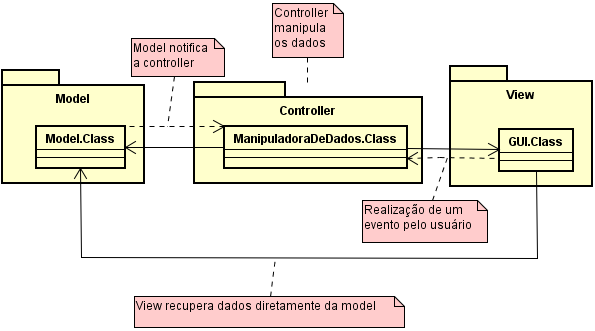
\includegraphics[keepaspectratio=true,scale=0.9]{figuras/DiagramaDeClasseMVC.PNG}
	\caption{Diagrama de classes representando a interação entre os componentes no padrão arquitetural MVC. Adaptado de \cite{durelli2008proposta}.}
	\label{DiagramaDeClasseMVC}
\end{figure}

\pagebreak

A Figura \ref{DiagramaDeSequenciaMVC} é um diagrama de sequência que representa o fluxo dos eventos em um cenário exemplo, onde a \textit{Controller} interage diretamente com a \textit{Model} e \textit{View}, onde o usuário entra com alguma informação e aguarda o retorno da aplicação. 


\begin{figure}[h!]
	\centering
	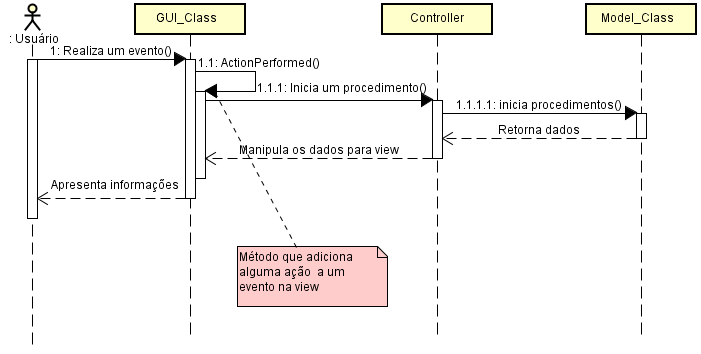
\includegraphics[keepaspectratio=true,scale=0.8]{figuras/DiagramaDeSequenciaMVC.PNG}
	\caption{Diagrama de sequência para o padrão arquitetural MVC. Adaptado de \cite{durelli2008proposta} e \cite{buschmann1996system}.}
	\label{DiagramaDeSequenciaMVC}
\end{figure}

\pagebreak

\section{Requisitos de segurança como RNFs}
\label{sec:seguranca}

Os RNFs de segurança podem ser entendidos como restrições, que realizam operacionalizações e satisfazem as metas de segurança, estabelecidas pelos engenheiros de requisitos e/ou engenheiros de software. Esse conjunto de  RNFs devem expressar de maneira precisa e não ambígua as metas de segurança de uma aplicação, fornecendo uma especificação para alcançar a meta deseja \cite{haley2006framework}.  

Existem diversas definições de segurança, de forma simplificada, segurança no contexto de segurança da informação, significa proteger a informação \cite{chung2012non}. Está monografia, portanto se fundamenta nos conceitos de \cite{chung2012non} e \cite{sullivan2011web} como base para para conceituar segurança, tomando como base os três conceitos conhecidos como CIA (\textit{Confidentiality}, \textit{Integrity}, \textit{Availability}) . 

Portanto, para a definição seguindo os fundamentos de \cite{chung2012non}, segurança se baseia em três conceitos, sendo eles: 

\begin{itemize}
	\item \textbf{Confidencialidade} (do inglês, \textit{Confidenciality}): Proteção da informação para evitar que as informações armazenadas ou transmitidas não poderão ser vistas ou interpretadas por terceiros, sendo somente o usuário principal e o destinatário. Promovendo essa proteção da informação através de algoritmos de criptografia \cite{chung2012non} \cite{silva2007arquitetura}. 
	
	\item \textbf{Integridade} (do inglês, \textit{Integrity}): Proteção contra qualquer tipo de atualização e/ou adulteração não autorizada, certifica-se que essa proteção seja garantida contra todo tipo modificação acidental ou maliciosa, garantindo então que a informação percorra, todo o trajeto entre o usuário principal e um destinatário \cite{chung2012non} \cite{silva2007arquitetura}. 
	
	\item \textbf{Disponibilidade} (do inglês, \textit{Availability}): Proteção contra a interrupção do serviço, no momento em que o usuário principal estiver necessitando da utilização do serviço \cite{chung2012non} \cite{silva2007arquitetura}.
	  
\end{itemize}


O CIA pode ser abstraído em metas flexíveis de segurança, logo depois, capturados e organizados em um catálogo de segurança, promovendo um conjunto rico de alternativas e pontos de verificação para se proteger contra a negligencia de pontos relevantes, e para a segurança da informação em uma aplicação. Como apresentado na Figura \ref{catalogoSegurancaChung}, onde abaixo, de cada conceito chave para segurança exitem seus subtipos. 

Apresentados em  verde na Figura \ref{catalogoSegurancaChung} estão outras características dos requisitos de segurança, sendo um dos mais relevantes o ``operacional``, que possui como subtipo ``segurança operacional`` que refere-se diretamente a segurança da informação \cite{chung2012non}.

Os subtipos das ``características dos RNF`` de acordo com \cite{chung2012non} podem ser ``ciclo de vida``, ``operacional \footnote[1]{Operação realizada por uma aplicação de software em tempo de execução \cite{chung2012non}.}``, ``desenvolvimento \footnote[2]{Estágios de desenvolvimento \cite{chung2012non}.}``, ``interna-externa \footnote[3]{Refere-se a confidencialidade dos itens de informação do sistema \cite{chung2012non}.}``, ``interna `` e ``externa``.

\begin{figure}[h!]
	\centering
	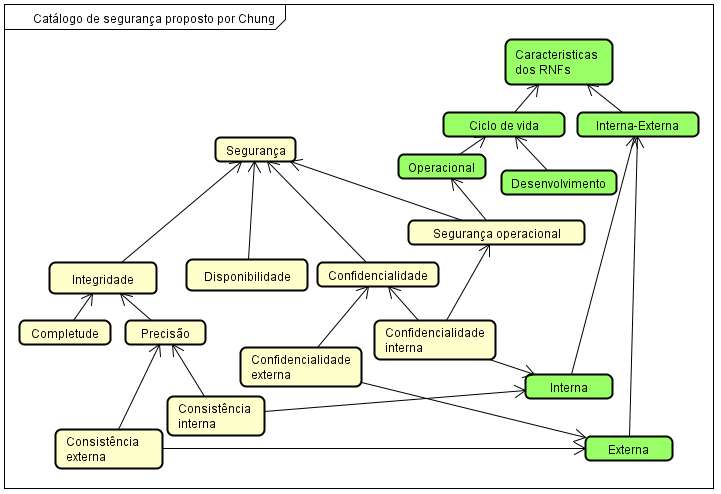
\includegraphics[keepaspectratio=true,scale=0.9]{figuras/catalogoSegurancaChung.PNG}
	\caption{Catálogo de segurança. Fonte: \cite{chung2012non}.}
	\label{catalogoSegurancaChung}
\end{figure}

É de extrema importância entender os conceitos na literatura dos subtipos de cada conceito, as subseções a seguir fazem um breve detalhamento sobre esses conceitos Confidencialidade e Integridade. 

\subsection{Confidencialidade}
\label{subsec:confidencialidade}

Se tratando de confidencialidade em \cite{reis10classificaccao} é definido conceitos sobre o tipo da informação em segurança, sendo eles: 

\begin{itemize}
	\item \textbf{Irrestrido}: Tipo de informação pública. 
	
	\item \textbf{Interna}: Tipo de informação que seu acesso deve ser evitada por público externo, caso este tipo de informação seja disponibilizada, por erro interno ou por ataque malicioso não causa nenhum impacto ao mantenedor da informação.
	
	\item \textbf{Confidencial}: Tipo de informação interna, onde, a disponibilidade ao público externo, por erro interno ou por ataque malicioso pode gerar vantagens a concorrentes e perda de usuários/clientes. 
	
	\item \textbf{Secreta}: Tipo de informação interna, restrita a um conjunto específico de usuários, onde, a disponibilidade tanto ao público externo quando ao público interno não definido, pode causar grandes danos. A integridade dessa informação deve ser mantida a qualquer custo.
\end{itemize} 

A confidencialidade possui os subtipos ``confidencialidade interna`` e ``confidencialidade externa`` de acordo com a Figura \ref{catalogoSegurancaChung}.
 

\subsection{Integridade}
\label{subsec:integridade}
 
Definida através dos conceitos precisão e completude, por \cite{chung2012non}, onde: 

\textbf{Precisão}: Pode ser entendida como qualquer atributo semântico, que fundamenta uma informação \cite{chung2012non}, ou seja, a garantia que um requisito da informação seja descrito com precisão de acordo com, suas especificações. 

\begin{itemize}
	\item \textbf{Propriedade da precisão}: Garantir que objetos sejam instanciados da maneira correta. 
	
	\item \textbf{Valor de precisão}: Garantir que os valores retornados pelas operações possuem a precisão desejada.
	
	\item \textbf{Precisão de um para um}: Garantir que um único objeto esteja ligado a uma única entidade do domínio. 
	
	\item \textbf{Consistência interna}: Garantir que os valores do mundo real seja correspondente aos valores do sistema.
\end{itemize}

\textbf{Completude}: Garantir que o RNF esteja completo \cite{chung2012non}. 

\section{Resumo do capítulo}

Neste Capítulo, foi abordado os conceitos fundamentais para a construção do catálogo de segurança, foi introduzidos os conceitos chaves da Engenharia de Requisitos e aprofundando em uma de suas áreas que é a Engenharia de Requisitos Orientada à Meta, para compreendermos o conceito de meta e as suas responsabilidades, partimos então para uma visão dos requisitos, focando somente nos requisitos não-funcionais, logo em seguida foi apresentado as características e notações dos modelos intencionais NFR \textit{Framework} e o i*, bem como a apresentação do FURPS. 

Os conceitos de arquitetura de software também, foram apresentados neste Capítulo, pois são de extrema importância, para o entendimento do padrão arquitetural MVC, ao qual o catálogo de segurança é voltado, Por fim foi apresentado a visão dos requisitos de segurança como RNFs, onde foi apresentado os conceitos chave e suas definições na área de segurança, para a construção do catálogo. 



\chapter{Suporte Tecnológico}
\label{chap:suporteTecnologico}

Neste Capítulo, é apresentado as ferramentas de software utilizadas para dar suporte ao desenvolvimento da monografia. A seção \ref{sec:ferramentasModelagem}, apresenta uma breve descrição das ferramentas utilizadas na modelagem dos diagramas e mapas mentais presentes na monografia e a seção \ref{sec:ferramentasDesenvolvimento} apresenta as ferramentas de suporte à escrita, e para a realização do controle de versão. 

\section{Ferramentas de modelagem}
\label{sec:ferramentasModelagem}

\begin{itemize}
	\item \textbf{Astah Professional}: é uma ferramenta de modelagem de diagramas dinâmicos e estáticos, que suporta a UML 2.x, \textit{Entity Relationship Diagram} (ERD), 
	
	\textit{Data Flow Diagram} (DFD), fluxogramas, mapas mentais, suportando a engenharia reversa para as linguagens Java, C\# e C++ \cite{astah}. A versão utilizada foi a v7.2.0 com licença de estudante, para modelagem dos diagramas da UML e mapas mentais.   
	
	\item \textbf{StarUML}: É um software \textit{open source} para modelagem de diagramas, para a UML/\textit{Model Driven Architecture} (MDA). A proposta da ferramenta e se tornar uma ferramenta gratuita que substitua as plataformas comerciais \cite{starUML}. A versão utilizada é a versão v1.0, pois suporta o \textit{plug-in} RE-Tools, que permite a modelagem do SIGs para o NFR Framework. 
	
	\item \textbf{OpenOME}: É uma ferramenta \textit{open source} de modelagem para apoiar a engenharia requisitos orientada à meta, orientada à agente e orientada à aspectos, ela promove ao desenvolvedor um vinculo entre os requisitos e as especificações e as fases do \textit{design} arquitetural \cite{openOME}. A versão utilizada é a v3.4.1, para modelagem na notação do i*. 
	
	\item \textbf{Xmind}: É um software proprietário para criação de mapas mentais e suporte na criação de \textit{brainstorming} \cite{xMind}. A versão utilizada é o XMind 8 Update 2, permitindo a criação de mapas mentais. 
	
	\item \textbf{Bizagi Modeler}: É uma ferramenta gratuita utilizada para modelagem de processos de negócio, utilizando notação BPMN. É eleita pela comunidade a mais potente e fácil de utilizar do mercado. A versão utilizada é a versão 3.1, para a modelagem do processo de desenvolvimento da monografia \cite{bizagi}. 
	
	\item \textbf{RE-Tools}: É um conjunto de ferramentas \textit{open source} utilizado para a modelagem de diferentes aspectos das organizações e de seus sistemas, durante a realização das atividades da engenharia de requisitos, possuindo suporte para as notações do (i) NFR Framework, (ii) i*, (iii) \textit{Knowledge Acquisition in autOmated Specification} (KAOS), (iv) \textit{Problem Frames}, (v) UML e (vi) BPMN \cite{reTools} \cite{supakkul2012re}.
	
	Esse conjunto de ferramentas vem sendo utilizado para o ensino da Engenharia de Requisitos em cursos na Universidade de Trento (Itália), Universidade do Texas em Dallas (Estados Unidos) e na Universidade de Brasília (Brasil), além de estar envolvida em pesquisas no Brasil, Austrália, Canadá, China, França, Reino Unido e Estados Unidos \cite{supakkul2012re}. 
	
	Na monografia a versão do \textit{plug-in} utilizada foi a v3.0.2, para modelagem do gráfico de SIGs. 
\end{itemize}

\section{Ferramentas para desenvolvimento da monografia}
\label{sec:ferramentasDesenvolvimento}

\begin{itemize}
	\item \textbf{Git}: É um sistema \textit{open source} que suporta o controle de versão distribuído \cite{git}. Utilizado para realizar o controle de versão da parte escrita da monografia. 
	\item \textbf{GitHub}: O GitHub é uma plataforma de hospedagem de código para controle de versão utilizando o Git, através do GitHub é possível criar uma conta para armazenar o código fonte de projetos em repositórios gratuitos e privados \cite{github}. Utilizado para hospedar o repositório público para o controle de versão da monografia. 
	\item \LaTeX\ : É um sistema que permite a elaboração de textos em alta qualidade, através do programa de diagramação de textos TEX \cite{latex}. Utilizado no desenvolvimento da parte escrita da monografia. 
\end{itemize}

\section{Resumo do capítulo}

Neste Capítulo foi descrito todas as ferramentas que deram suporte para a escrita o desenvolvimento dessa monografia. Na seção \ref{sec:ferramentasModelagem} foi apresentada as versões e a utilização de cada ferramenta, e a seção \ref{sec:ferramentasDesenvolvimento} apresenta as ferramentas utilizadas no desenvolvimento da parte escrita e o controle de versão da mesma. 

\chapter{Metodologia}
\label{chap:metodologia}

Neste Capítulo, é apresentado a classificação de pesquisa na secção \ref{sec:classificacaoDaPesquisa}, onde detalha-se a pesquisa de acordo com seus tipos de classificações como abordagem de pesquisa, natureza de pesquisa, objetivos de pesquisa e procedimentos técnicos de pesquisa. E a seção \ref{sec:procedimentosMetodológicos} apresenta os procedimentos metodológicos para o desenvolvimento dessa monografia, onde detalha-se o fluxo de atividades e o cronograma seguido tanto para o TCC1 e TCC2.  

\section{Classificação da pesquisa}
\label{sec:classificacaoDaPesquisa}

A pesquisa científica pode ser classificada de acordo com sua abordagem, sua natureza, seus objetivos e seus procedimentos técnicos \cite{gerhardt2009metodos}. O objetivo desta seção é detalhar os tipos de classificações de pesquisa utilizados no desenvolvimento desta monografia. 

\subsection{Abordagem de pesquisa}

Segundo \cite{gerhardt2009metodos}, a pesquisa qualitativa preocupa-se com os aspectos da realidade e que não podem ser quantificados, centrando-se na compreensão e explicação da dinâmica das relações sociais. Também possui três características fundamentais para prosseguir com os estudos \cite{mazzotti1991planejamento}, são elas:

\begin{itemize}
	\item \textit{Visão Holística:} Onde a compreensão de um comportamento ou evento só é possível com o entendimento das inter-relações que surgem dentro do contexto da pesquisa;
	\item \textit{Abordagem indutiva:} Onde o pesquisador parte de observações mais livres deixando que as dimensões e categorias de interesse surjam progressivamente durante todo o processo de coleta e análise dos dados;
	\item \textit{Investigação naturalística:} Onde a intervenção do pesquisador no contexto observado é reduzida ao mínimo.
\end{itemize}

A abordagem de \textbf{pesquisa qualitativa} é utilizada na execução desta pesquisa, pois para execução da pesquisa, o autor tem a necessidade de realizar as ações de descrever os principais subtipos de RNFs de segurança, para estruturação de um catálogo de segurança utilizando o NFR \textit{Framework}, bem como compreender e explicar os impactos entre os RNFs no padrão arquitetural MVC. 

\subsection{Natureza de pesquisa}

Essa pesquisa é caracterizada como uma \textbf{pesquisa aplicada}, pois os conhecimentos gerados são voltados para a aplicação prática \cite{gerhardt2009metodos}, voltados à solução de como auxiliar os engenheiros de requisitos e engenheiros de software na especificação dos RNFs de segurança, quando uma arquitetura é imposta. 

\subsection{Objetivos de pesquisa}

Com base no objetivo de pesquisa é possível classificar essa pesquisa como \textbf{pesquisa explicativa}, pois de segundo \cite{gil2002elaborar} “..este tipo de pesquisa preocupa-se em identificar os fatores que determinam ou que contribuem para a ocorrência dos fenômenos..”, ou seja, na presente pesquisa pretende-se explicar como o padrão arquitetural MVC pode ser impactado pelos RNFs, de acordo com o catálogo de segurança.

\subsection{Procedimentos técnicos de pesquisa}

A \textbf{pesquisa bibliográfica} é um dos procedimentos técnicos de pesquisa utilizado, como é evidente no Capítulo \ref{chap:referencialTeorico}, onde é apresentado todo o levantamento teórico que serve de insumo para a execução dessa monografia. De acordo com \cite[p.35]{fonseca2002metodologia} “\textit{esse tipo de procedimento trata-se do levantamento de referências teóricas já analisadas, e publicadas por meio de escritos e eletrônicos, como livros, artigos científicos, páginas de web sites. Qualquer trabalho científico inicia-se com uma pesquisa bibliográfica, que permite ao pesquisador conhecer o que já estudou sobre o assunto}“.
 
Outro procedimento técnico de pesquisa adotado é a \textbf{pesquisa ação}, pois se trata de uma participação planejada do ator em uma situação problemática a ser investigada \cite{fonseca2002metodologia}. O ator participa ativamente do levantamento adquirindo consigo uma série de conhecimentos que servirão como base para construção do catálogo de segurança e que em tempo de execução do TCC2 será validado, através do desenvolvimento de uma solução de software utilizando o padrão arquitetural MVC. 

\section{Procedimentos Metodológicos}
\label{sec:procedimentosMetodológicos}

Para o desenvolvimento da monografia foi realizado várias atividades, essas atividades foram então organizadas como um processo de desenvolvimento da monografia. Como apresentado nas Figuras \ref{PDM-TCC1} e \ref{PDM-TCC2}. 

Pelas diretrizes do curso de graduação em Engenharia de Software é necessário à aprovação nas disciplinas de TCC1 e TCC2, logo as próximas seções detalham o fluxo de execução de atividades para concluir a monografia. 



\subsection{Processo de desenvolvimento da monografia para o TCC1}

Este processo tem como principal objetivo a elaboração e estruturação do catálogo de segurança para o padrão arquitetural MVC. 

\begin{figure}[h!]
	\centering
	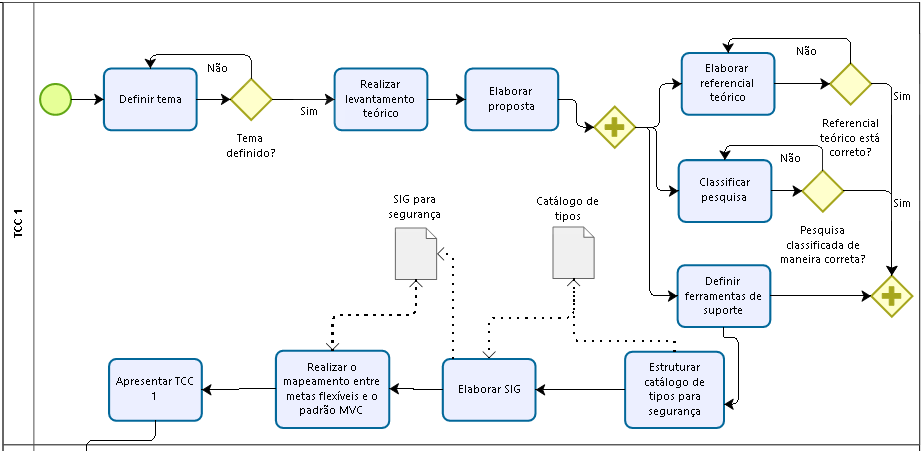
\includegraphics[keepaspectratio=true,scale=0.6]{figuras/PDM-TCC1.PNG}
	\caption{Atividades do processo de desenvolvimento da monografia para o TCC1.}
	\label{PDM-TCC1}
\end{figure}

As atividades são:

\begin{itemize}
	\item \textbf{Definir tema}: Junto com os professores orientadores dessa monografia, essa atividade teve, como principal objetivo o refinamento sobre os conceitos teóricos, referente a área de interesse do autor.   
	
	\item \textbf{Realizar levantamento teórico}: Com base nos resultados obtidos da execução da atividade anterior, iniciou-se o levantamento teórico, com base nas orientações dos orientadores. Onde foi discutido os aspectos fundamentais do GORE, os \textit{frameworks} se se apoiam nos conceitos do GORE, conceitos de Arquitetura de Software e sobre os atributos de qualidade mais relevantes para o mercado e para a academia. 
	
	\item \textbf{Elaborar proposta}: Com o conhecimento das necessidades da área de atuação dessa monografia, iniciou a elaboração da proposta de pequisa, junto aos orientados, onde foi discutido e acordado a utilização do NFR \textit{Framework} e a decisão de aplicar o trabalho ao mercado, tomando como \textbf{segurança} sendo o atributo de qualidade mais relevante.  
	
	\item \textbf{Elaborar referencial teórico}: Redação dos conceitos teóricos a serem aplicados no desenvolvimento da monografia. 
	
	\item \textbf{Classificar pesquisa}: Redação  da classificação da pesquisa em suas dimensões em (i) abordagem de pesquisa,  (ii) natureza de pesquisa, (iii) objetivos de pesquisa e os (iv) procedimentos técnicos de pesquisa.  
	
	\item \textbf{Definir ferramentas de suporte}: Definição e descrição das ferramentas utilizadas no desenvolvimento da monografia.  
	
	\item \textbf{Estruturar catálogo de tipos de segurança}: Com base nos conceitos de segurança apresentados por Lawrence Chung, Brian A. Nixon, Eric Yu e John Mylopoulos no  livro: \textit{NON-FUNCTIONAL REQUIREMENTS
	IN SOFTWARE ENGINEERING}, iniciou a elaboraçao  do catálogo de tipos de RNFs para segurança, e expandindo o catálogo com base em definições de subtipos de RNFs de segurança definidos por outros autores.
	
	\item \textbf{Elaborar SIG}: A partir do catálogo de segurança, iniciou-se o processo de identificação das metas flexíveis que podem ser satisfeitas e fundamentando em alguns exemplos do livro: \textit{NON-FUNCTIONAL REQUIREMENTS IN SOFTWARE ENGINEERING}.
	
	\item \textbf{Realizar o mapeamento entre metas flexíveis e o padrão MVC}: Iniciou-se a comparação das metas flexíveis que possuiam, tipo arquitetural e gerariam impactos positivos ou negativos, na segurança dos dados e da arquitetura. 
	
	\item \textbf{Apresentar TCC 1}: Defesa do TCC1 para a banca. 
\end{itemize}

\subsection{Processo de desenvolvimento da monografia para o TCC2}

Este processo tem como principal objetivo a validação do catálogo proposto, através do desenvolvimento de uma aplicação de software. 

As atividades são:

\begin{figure}[h!]
	\centering
	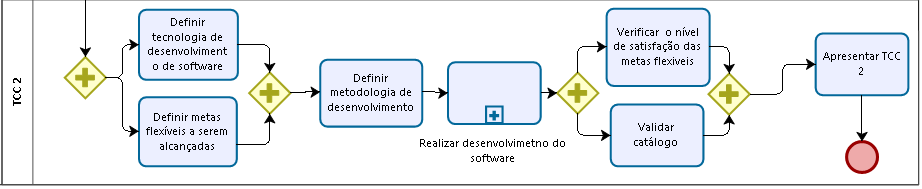
\includegraphics[keepaspectratio=true,scale=0.7]{figuras/PDM-TCC2.PNG}
	\caption{Atividades do processo de desenvolvimento da monografia para o TCC2.}
	\label{PDM-TCC2}
\end{figure}

\begin{itemize}
	\item \textbf{Definir tecnologia de desenvolvimento de software}: Definir ferramentas para o desenvolvimento do software de exemplo, desenvolvido utilizando o padrão arquitetural MVC.
	
	\item \textbf{Definir metas flexíveis a serem alcançadas}: Definir as metas flexíveis a serem alcançadas de acordo com o cenário exemplo do software a ser desenvolvido.
	
	\item \textbf{Definir metodologia de desenvolvimento}: Definir metodologia de desenvolvimento de software a ser utilizada.  
	
	\item \textbf{Macro atividade: Realizar desenvolvimento do software}: Realizar as etapas de desenvolvimento de acordo com a metodologia selecionada.
	
	\item \textbf{Verificar o nível de satisfação das metas flexíveis}: Verificar se as metas flexíveis foram alcançadas após o desenvolvimento do software
	
	\item \textbf{Validar catálogo}: Validar o catálogo de segurança porposto no TCC1 de acordo com o cenário especificado. 
	
	\item \textbf{Apresentar TCC 2}: Apresentar TCC 2 para a banca.
\end{itemize}

\subsection{Cronograma das atividades de desenvolvimento da monografia}

O planejamento com os meses de execução de cada atividade do processo de desenvolvimento da monografia seguem nas Tabelas \ref{cronograma-tcc1} e \ref{cronograma-tcc2} respectivamente. 

\begin{table}[h!]
	\centering
	\caption{Cronograma das atividades para desenvolvimento do TCC1.}
	\label{cronograma-tcc1}
	\begin{tabular}{|l|c|c|c|c|c|c|c|}
		\hline
		\textbf{Atividade} & \multicolumn{1}{l|}{\textbf{Ago}} & \multicolumn{1}{l|}{\textbf{Set}} & \multicolumn{1}{l|}{\textbf{Out}} & \multicolumn{1}{l|}{\textbf{Nov}} & \multicolumn{1}{l|}{\textbf{Dez}} & \multicolumn{1}{l|}{\textbf{Jan}} & \multicolumn{1}{l|}{\textbf{Fev}} \\ \hline
		Definir tema & \textbf{x} & \textbf{} & \textbf{} & \textbf{} & \textbf{} & \textbf{} & \textbf{} \\ \hline
		Realizar levantamento teórico & \textbf{x} & \textbf{x} & \textbf{} & \textbf{} & \textbf{} & \textbf{} & \textbf{} \\ \hline
		Elaborar proposta & \textbf{x} & \textbf{x} & \textbf{x} & \textbf{} & \textbf{} & \textbf{} & \textbf{} \\ \hline
		Elaborar referencial teórico & \textbf{} & \textbf{} & \textbf{x} & \textbf{x} & \textbf{x} & \textbf{} & \textbf{} \\ \hline
		Classificar pesquisa & \textbf{} & \textbf{} & \textbf{x} & \textbf{x} & \textbf{x} & \textbf{} & \textbf{} \\ \hline
		Definir ferramentas de suporte & \textbf{} & \textbf{} & \textbf{x} & \textbf{x} & \textbf{x} & \textbf{} & \textbf{} \\ \hline
		\begin{tabular}[c]{@{}l@{}}Estruturar catálogo de tipos \\ para segurança\end{tabular} & \textbf{} & \textbf{} & \textbf{} & \textbf{} & \textbf{x} & \textbf{x} & \textbf{} \\ \hline
		Elaborar SIG & \textbf{} & \textbf{} & \textbf{} & \textbf{} & \textbf{x} & \textbf{x} & \textbf{} \\ \hline
		\begin{tabular}[c]{@{}l@{}}Realizar mapeamento entre metas\\ flexíveis e o padrão MVC\end{tabular} & \textbf{} & \textbf{} & \textbf{} & \textbf{} & \textbf{} & \textbf{x} & \textbf{x} \\ \hline
		Apresentar TCC1 & \textbf{} & \textbf{} & \textbf{} & \textbf{} & \textbf{} & \textbf{} & \textbf{x} \\ \hline
	\end{tabular}
\end{table}

\begin{table}[h!]
	\centering
	\caption{Cronograma das atividades para desenvolvimento do TCC2.}
	\label{cronograma-tcc2}
	\begin{tabular}{|l|c|c|c|c|c|}
		\hline
		\textbf{Atividade} & \multicolumn{1}{l|}{\textbf{Mar}} & \multicolumn{1}{l|}{\textbf{Abr}} & \multicolumn{1}{l|}{\textbf{Mai}} & \multicolumn{1}{l|}{\textbf{Jun}} & \multicolumn{1}{l|}{\textbf{Jul}} \\ \hline
		\begin{tabular}[c]{@{}l@{}}Definir tecnologia de desenvolvimento\\ de software\end{tabular} & \textbf{x} & \textbf{} & \textbf{} & \textbf{} & \textbf{} \\ \hline
		Definir metas flexíveis a serem alcançadas & \textbf{x} & \textbf{} & \textbf{} & \textbf{} & \textbf{} \\ \hline
		Definir metodologia de desenvolvimento & \textbf{x} & \textbf{x} & \textbf{} & \textbf{} & \textbf{} \\ \hline
		Realizar desenvolvimento do software & \textbf{} & \textbf{x} & \textbf{x} & \textbf{x} & \textbf{} \\ \hline
		\begin{tabular}[c]{@{}l@{}}Verificar o nível de satisfação das metas\\ flexíveis\end{tabular} & \textbf{} & \textbf{} & \textbf{x} & \textbf{x} & \textbf{} \\ \hline
		Validar catálogo & \textbf{} & \textbf{} & \textbf{} & \textbf{x} & \textbf{} \\ \hline
		Apresentar TCC 2 & \textbf{} & \textbf{} & \textbf{} & \textbf{} & \textbf{x} \\ \hline
	\end{tabular}
\end{table}

\section{Resumo do capítulo}

Neste capitulo foi detalhada a classificação da pesquisa de acordo com seus tipos, como sendo a (i) abordagem de pesquisa, se tratando de uma pesquisa qualitativa, a (ii) Natureza de pesquisa, caraterizada como uma pesquisa aplicada, o (ii) objetivo de pesquisa, caracterizado como uma pesquisa explicativa e os (iv) procedimentos técnicos de pesquisa, caracterizados como uma pesquisa bibliográfica e a pesquisa ação. Também foi detalhado o fluxo de atividades para o desenvolvimento dessa monografia englobando a sua execução para a execução das disciplinas obrigatórias TCC1 e TCC2.

\chapter{Proposta}
\label{chap:proposta}



\section{Catálogo de tipos de RNFs para segurança}

Um catálogo de tipos de segurança promove a engenheiros de requisitos e engenheiros de software, o entendimento das diferentes necessidades, se tratando dos domínios de segurança dos dados e segurança arquitetural de uma aplicação de software. Pois com base no catálogo, pode se escolher os conceitos de segurança que são mais relevantes para o desenvolvimento da aplicação.

A Figura \ref{catalogoDeTipos} apresenta o catálogo de tipos de segurança proposto por esta monografia, nele as caraterísticas externas dos RNFs de segurança foram descartadas, pois a presente monografia trata apenas como o mundo real pode prejudicar o software em questões arquiteturais, e que podem ou não gerar impacto sobre os consistência dos dados.    

As cores no catálogo são para facilitar o entendimento e identificar de onde, vem RNF mais genérico. 

\begin{figure}[h!]
	\centering
	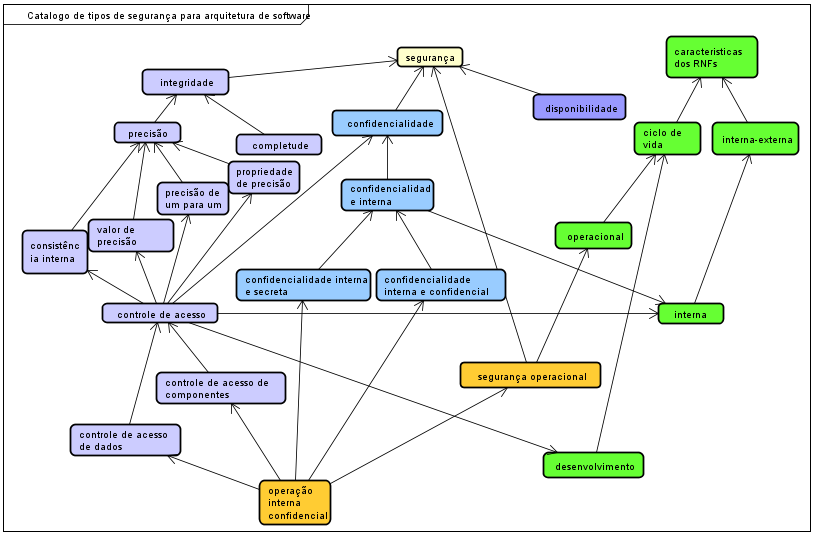
\includegraphics[keepaspectratio=true,scale=0.8]{figuras/catalogoDeTiposSeguranca.PNG}
	\caption{Catálogo de tipos para segurança arquitetural de software.}
	\label{catalogoDeTipos}
\end{figure}

Para ``disponibilidade`` apresentado em roxo escuto escuro na Figura \ref{catalogoDeTipos}, se trata da proteção contra a interrupção dos serviços em execução, no momento em que o usuário estiver utilizando a aplicação, visando a disponibilidade das funções internas dentro da própria arquitetura do software. 

Já em ``segurança operacional`` apresentado em laranjado na Figura \ref{catalogoDeTipos} e seu subtipo ``operação interna confidencial`` referindo-se diretamente a manutenção da segurança dos dados e componentes durante a execução do software. 

\subsection{Integridade}

Integridade e seus subtipos são representados no catálogo da Figura \ref{catalogoDeTipos} através da cor roxo claro. 

Como definido na Subseção \ref{subsec:integridade} integridade, pode ser abstraída em dois subtipos, precisão e completude, onde precisão pode ser abstraída em mais 4 subtipos \cite{chung2012non}, que são relevantes para a manutenção do controle de acesso de usuários e da própria permissão de instanciação de objetos dentro das camadas do padrão arquitetural MVC. 

O papel de cada RNF dentro do catálogo possui uma função específica, para ``precisão`` tem-se os subtipos, (i) ``propriedade de precisão``, cuja o papel dentro do catálogo é manter que um objeto não seja instanciado por uma classe em uma camada diferente ao qual no possui relação para tal, dentro do padrão arquitetural MVC, e de forma análoga o (ii) ``valor de precisão``, visa a garantia de que os valores retornados pelas operações possuem a precisão desejada, dentro de uma mesma camada, ou quando ocorre o retorno de uma função para uma outra função em outra camada no MVC, a (iii) ``precisão de um para um``, possui foco na \textit{model} pois, verifica se existe uma única entidade do mundo real, ligada a um objeto instanciado pela model. e (iv) ``consistência interna``, promover que os valores do mundo real sejam correspondente aos valores, e abstrações contidas no sistema (entidades, métodos, dados)

O RNF ``controle de acesso`` é uma especificidade de todas as especificidades de precisão, pois procura-se garantir a consistência e precisão nas dimensões de dados e componentes dentro do padrão arquitetural MVC. Portanto, as especificações desse RNF são juntamente (i) ``controle de acesso de dados`` e ``(ii) ``controle de acesso de componentes``.

Para ``completude`` é a garantia de que o RNFs esteja completo e não ambíguo.

\subsection{Confidencialidade}

Confidencialidade e seus subtipos são representados no catálogo da Figura \ref{catalogoDeTipos} através da cor azul. 

Como o foco é a parte arquitetural e como ocorrem os impactos entre os RNFs de segurança, para os aspectos de confidencialidade foram levados em considerações, somente os que possuíam relevância interna onde, ``confidencialidade interna``, trata-se dos termos, métodos, e instâncias de classes dentro do padrão MVC, que devem ser utilizamos somente dentro da aplicação, e um determinado ataque ou erro interno não prejudica o mantenedor da aplicação.

Para ``confidencialidade interna e secreta``, se aplica o mesmo conceito da ``confidencialidade interna``, exceto que a integridade da informação deve ser mantida a qualquer custo, e a ocorrência de um determinado ataque ou erro causa grandes danos em quem mantém a aplicação.

Para ``confidencialidade interna e confidencial``, aplica-se os mesmos conceitos das anteriores, exceto se a ocorrência de um determinado ataque ou erro pode causar vantagens a concorrentes, perda de usuários e clientes. 

\pagebreak

\section{Gráfico de interdependência entre metas flexíveis - SIGs}

Os subtipos de conceitos que compõem a definição de segurança são abstraídos e tratados como metas flexíveis, para então serem modelados e analisado o impacto entre eles, essa seção possui o intuito de detalhar cada nó do SIG, para isso o gráfico foi reduzido em pequenas partes, para facilitar o entendimento do leitor.

Entende-se no grafo o tipo [\textbf{dados}], as informações contidas nas bases de dados e os valores utilizados como parâmetros, e retornos de métodos dentro das camadas do padrão MVC. E o tipo [\textbf{arquitetural}], as estruturas dos componentes que compões o MVC. 

\begin{figure}[h!]
	\centering
	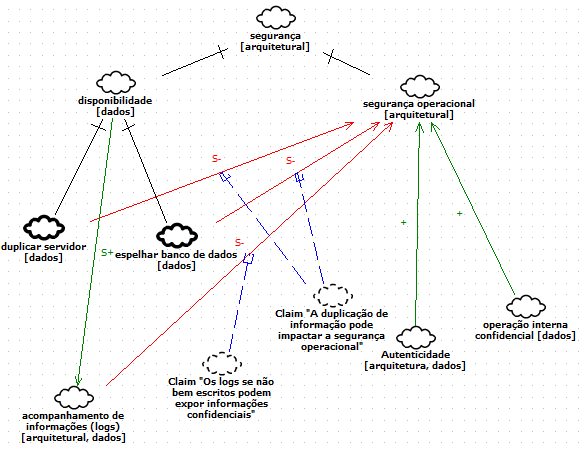
\includegraphics[keepaspectratio=true,scale=0.8]{figuras/SIG-SO-e-Disponibilidade.PNG}
	\caption{Decomposição de segurança para disponibilidade e segurança operancional}
	\label{DecomposicaoDisponibilidade}
\end{figure}

Como apresentado na Figura \ref{DecomposicaoDisponibilidade}, a de ``disponibildade[dados]`` pode ser decomposta em duas operacionalizações, baseado em \cite{affleck2012supporting}, e possui um \textit{link} de contribuição, representando uma contribuição positiva com ``acompanhamento de informações (\textit{logs}) [arquitetural,dados]``, pois a disponibilidade dos dados, podem constituir a geração dos \textit{logs}, tanto para verificação do comportamento entre os componentes dentro da arquitetura, quanto para as informações de entrada do usuário, logo a decomposição pode ser descrita pela expressão\footnote[1]{Os tipos de contribuições serão expressados no inglês conforme a Tabela \ref{tiposDeContribuições}.} \ref{eq:disponibilidade}.

\pagebreak

\begin{eqnarray}
\label{eq:disponibilidade}
\textrm{duplicar servidor[dados] AND}  \nonumber\\
\textrm{espelhar banco de dados[dados] AND} \nonumber \\
\textrm{SATISFAZ disponibilidade[dados]} 
\end{eqnarray}

e o impacto de ``disponibilidade[dados]`` sobre ``acompanhamento de informações(\textit{logs}) [arquitetural,dados]`` pela expressão


\begin{eqnarray}
\label{eq:disponibilidadeImpacto}
\textrm{disponibilidade[dados]}  \nonumber\\
\textrm{SOME+ acompanhamento de informações (logs)[arquitetural,dados]} 
\end{eqnarray}
\section{Resumo do capítulo}

\chapter{Considerações finais}
\label{chap:consideracoesFinais}